\section{Theorie}

Myonen werden in der Atmosphäre durch Kollision von Teilchen dort mit Protonen aus extragalaktischen Quellen erzeugt. Da sie sich mit relativistischer Geschwindigkeit bewegen, erreichen sie trotz ihrer kurzen Lebensdauer den Erdboden. Der Zerfall in ein Elektron und zwei Neutrinos kann mit Hilfe eines geeigneten Versuchsaufbaus gemessen und so die Lebensdauer der Myonen bestimmt werden.

\subsection{Eigenschaften von Myonen}

Durch die Kollision von Protonen aus extragalaktischen Quellen wie z. B. Supernova-Überresten und aktiven Galaxienkernen werden Pionen erzeugt, welche in Myonen und Antimyonen zerfallen. Mit einer durchschnittlichen Energie von \SI{4}{\mega\electronvolt}\cite{PGD}

\begin{figure}[h]
	\centering
	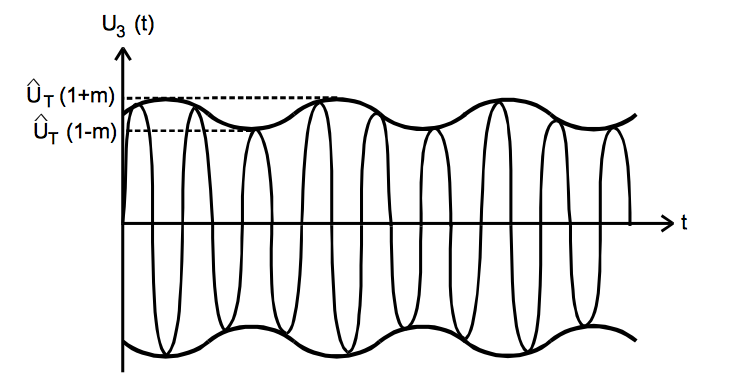
\includegraphics[width=\textwidth]{img/Abb1.png}
	\caption{Zeitabhängigkeit der Signalspannung eines Amplitudenmodulierten Signals \cite{FP}}
\end{figure}
